% for landscape posters, use "a4paper, landscape"
\documentclass[a4paper]{article}
\usepackage{better_poster}


% ---- fill in from here
% poster size - this will scale the poster to the given size.
% for landscape posters add ", landscape" to the postersize command.
\postersize{a0paper}

% authors
\title{Can Effective Invariance Metrics Predict Classifier Accuracy in a Data-Centric View?}
\author{Callum Koh}

% type of poster: [exp]erimental results, [methods], [theory]
% Disclaimer: the original classification had "study" and "intervention" as separate categories. I group them under experimental results.
\newcommand\postertype{empirical} % [exp],[methods],[theory]

\begin{document}

% main point of your study
\makefinding{
We're Investigating the \textbf{Relationship}\\ 
between \textbf{Image Classification Accuracy}\\ 
and \textbf{Other Self-Supervised/Unsupervised Metrics}.
}



% the main text of your poster goes here
\makemain{
    % you can have 1 or 2 columns
    \raggedcolumns
    \begin{multicols}{2}
        \section{Intro}
        \vspace{-0.3cm}
        \begin{compactitem}
            \item Image classification models require many images outside training to understand their generalisability.
            \item Adding labels to images is laborious and time-consuming.
            \item \textbf{Exists many reliable metrics} such as Rotation Invariance (RI) for \textbf{gauging image classification accuracy.}
            \item We \textbf{compare} above metrics \textbf{with our own jigsaw invariance} metric.
        \end{compactitem}
        \vspace{0.34cm}
        \begin{compactitem}
            \item CIFAR-10 dataset has 60,000 images, 1 of 10 unique objects in each.
            \item Includes planes, frogs, boats, etc.
            \item Small images promote simplicity in proof of concepts such as ours.
        \end{compactitem}
        \vspace{-0.4cm}
        \section{Data Used}
        \vspace{-0.3cm}
        \begin{compactitem}
            \item In-distribution (ID) CIFAR-10 test set + its copies via. image transforms,
            \item Various out-of-distribution (OOD) CIFAR-10 variants + its copies through image transforms.
        \end{compactitem}
        \vspace{-0.4cm}
        \section{Jigsaw Invariance (JI)}
        \begin{compactenum}
            \item Classifier takes image \(x\), outputting predicted class \(\hat{y}\) and confidence \(\hat{p}\).
            \item Turn \(x\) into jigsaw puzzle \(x_t\).
            \item Feed \(x_t\) into model, outputting associated \(\hat{y}_t\) and \(\hat{p}_t\).
            \item Same \(\hat{y}\) and \(\hat{y}_t\) with high \(\hat{p}\) and high \(\hat{p}_t\) implies high JI, and vice versa.
            \item Take mean average JI over all images \(x\) in dataset.
        \end{compactenum}
        
        
    % this determines where your columns will be separated
    \columnbreak
        \section{Results}
        \vspace{-0.3cm}
        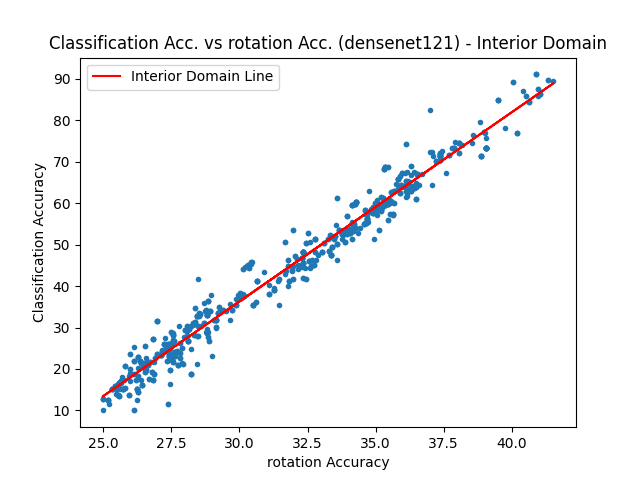
\includegraphics[scale=0.44]{images/sample1.png}
        \begin{compactitem}
            \item \textbf{No relationship between image classification accuracy and JI}, contrary to past observations.
            \item JI and RI derive from Effective Invariance (EI). Correlation shown only when dataset fixed + each point is a model (model-centric).
            \item CIFAR-10 uses 32 by 32 images - small size introduces biases.
        \end{compactitem}
        \vspace{-0.4cm}
        \section{Future Work}
        \vspace{-0.3cm}
        \begin{compactitem}
            \item Adopt model-centric view instead of dataset-centric,
            \item Use dataset with larger images, such as ImageNet,
            \item In this way possibly obtain better comparison between JI and other metrics.
        \end{compactitem}
    \end{multicols}
}
% If you have extra figures or data to show
\makeextracolumn{
    \begin{flushleft}
    Linear Classifier - Jigsaw (Simplest)
    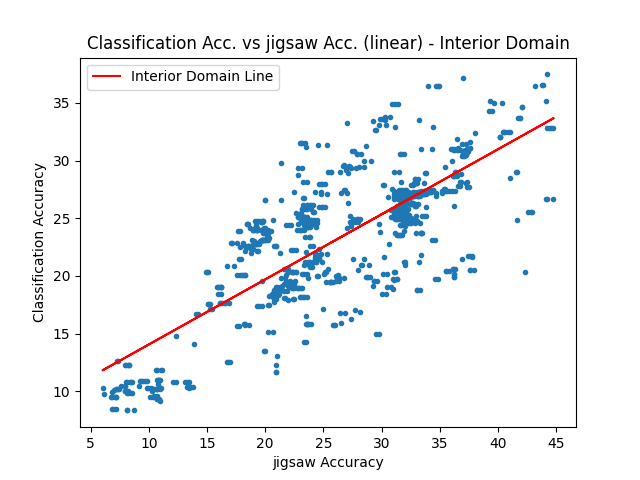
\includegraphics[scale=0.16]{images/sample3.png}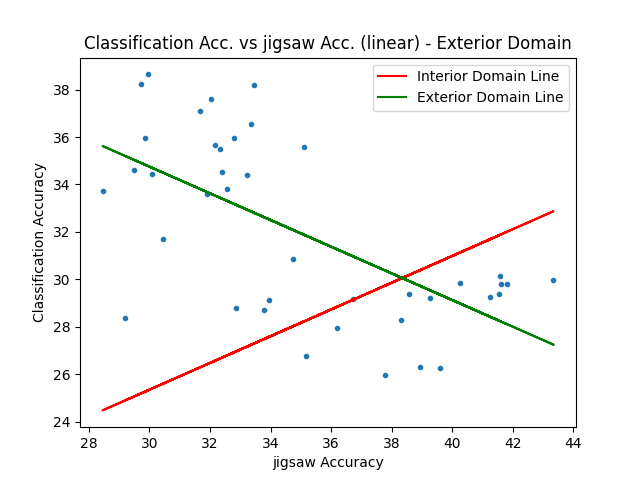
\includegraphics[scale=0.16]{images/sample2.png}
    LeNet5 - Jigsaw
    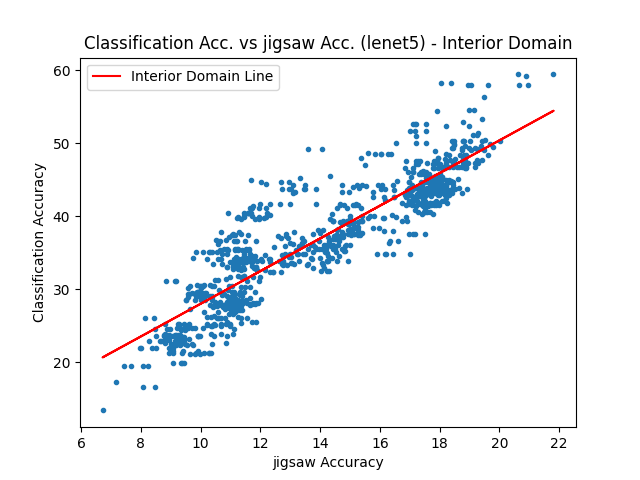
\includegraphics[scale=0.16]{images/sample8.png}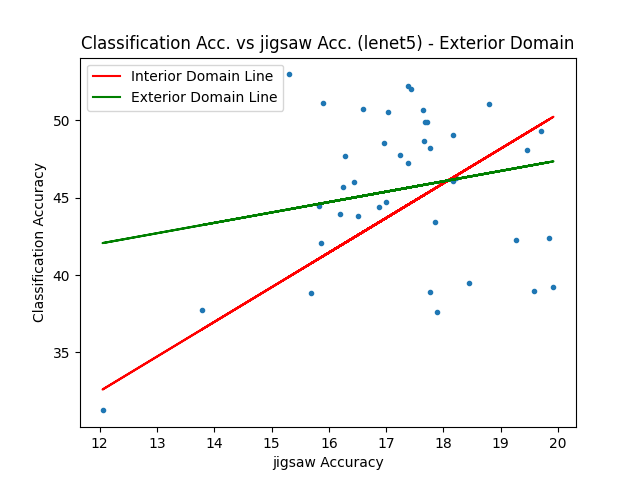
\includegraphics[scale=0.16]{images/sample9.png}
    ShuffleNet - Rotation
    \includegraphics[scale=0.16]{images/sample10.png}\includegraphics[scale=0.16]{images/sample11.png}
    Inception\_v3 - Rotation
    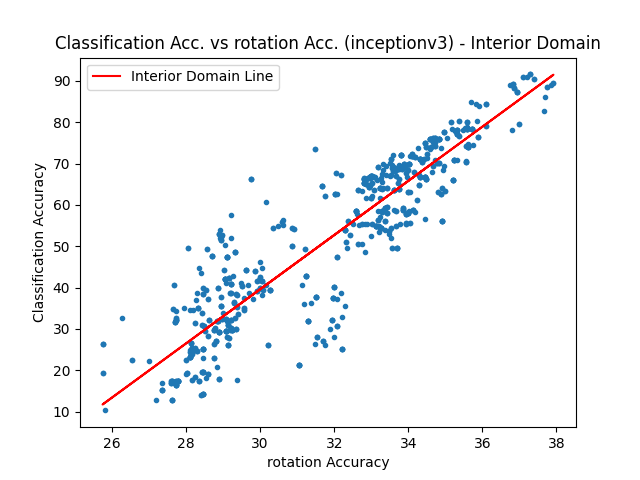
\includegraphics[scale=0.16]{images/sample4.png}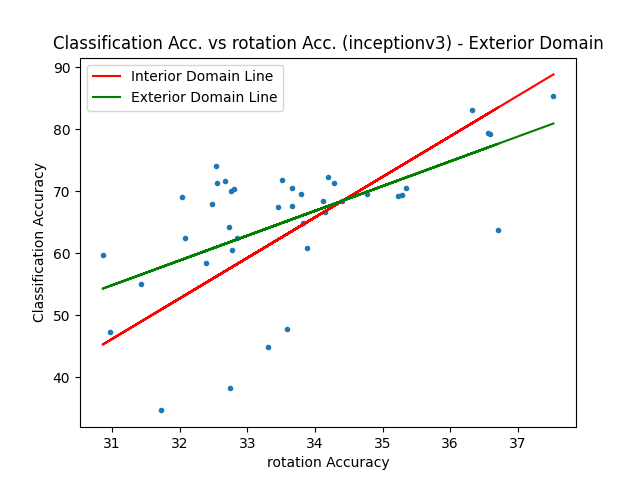
\includegraphics[scale=0.16]{images/sample5.png}
    DenseNet169 - Jigsaw
    \includegraphics[scale=0.16]{images/sample12.png}\includegraphics[scale=0.16]{images/sample13.png}
    ResNet1202 - Jigsaw (Most Complex)
    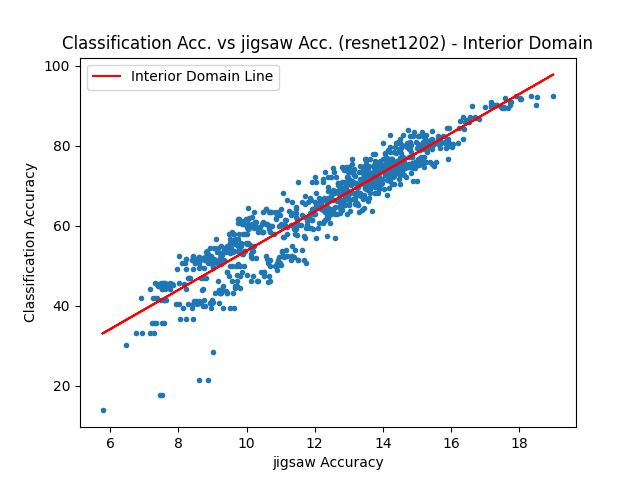
\includegraphics[scale=0.16]{images/sample6.png}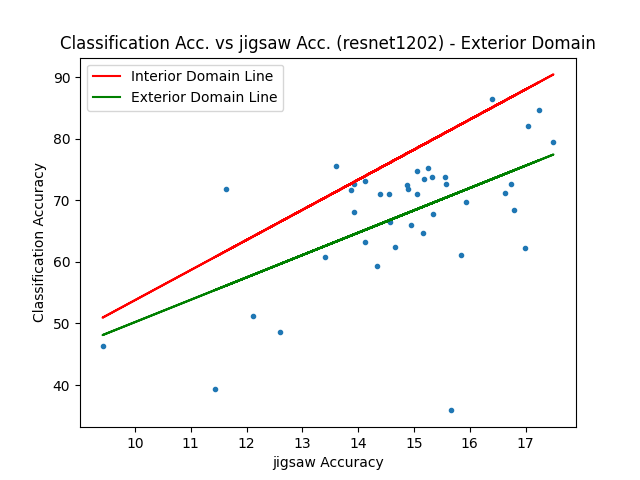
\includegraphics[scale=0.16]{images/sample7.png}

    \vspace{0.3cm}
    EI over a single image.
    \[
        \text{EI}(\hat{y},\hat{y}_t,\hat{p},\hat{p}_t) = \mathbf{1}(\hat{y}=\hat{y}_t)\sqrt{\hat{p}\cdot\hat{p}_t}
    \]
    EI for a whole dataset \(D\).
    \[
        \text{EI}_D = \frac{1}{|D|}\sum_{x \in D}EI(\hat{y},\hat{y}_t,\hat{p},\hat{p}_t)
    \]
    \end{flushleft}
}

% footer
% generate qr code from https://www.qr-code-generator.com/ and replace qr_code.png
% default: barcode on the left
\makefooter{images/uni_logo1.png}{images/paperqr.png}
\end{document}